
\begin{frame}{Cheating}
\framesubtitle{Theory}

        Intuivement, the cheater who would want to increase (or decrease) the reputation of one object in one characteristic would be tempted to simply rise his rating for this object and characteristic. But in theory...
        
        \begin{figure}
            \centering
            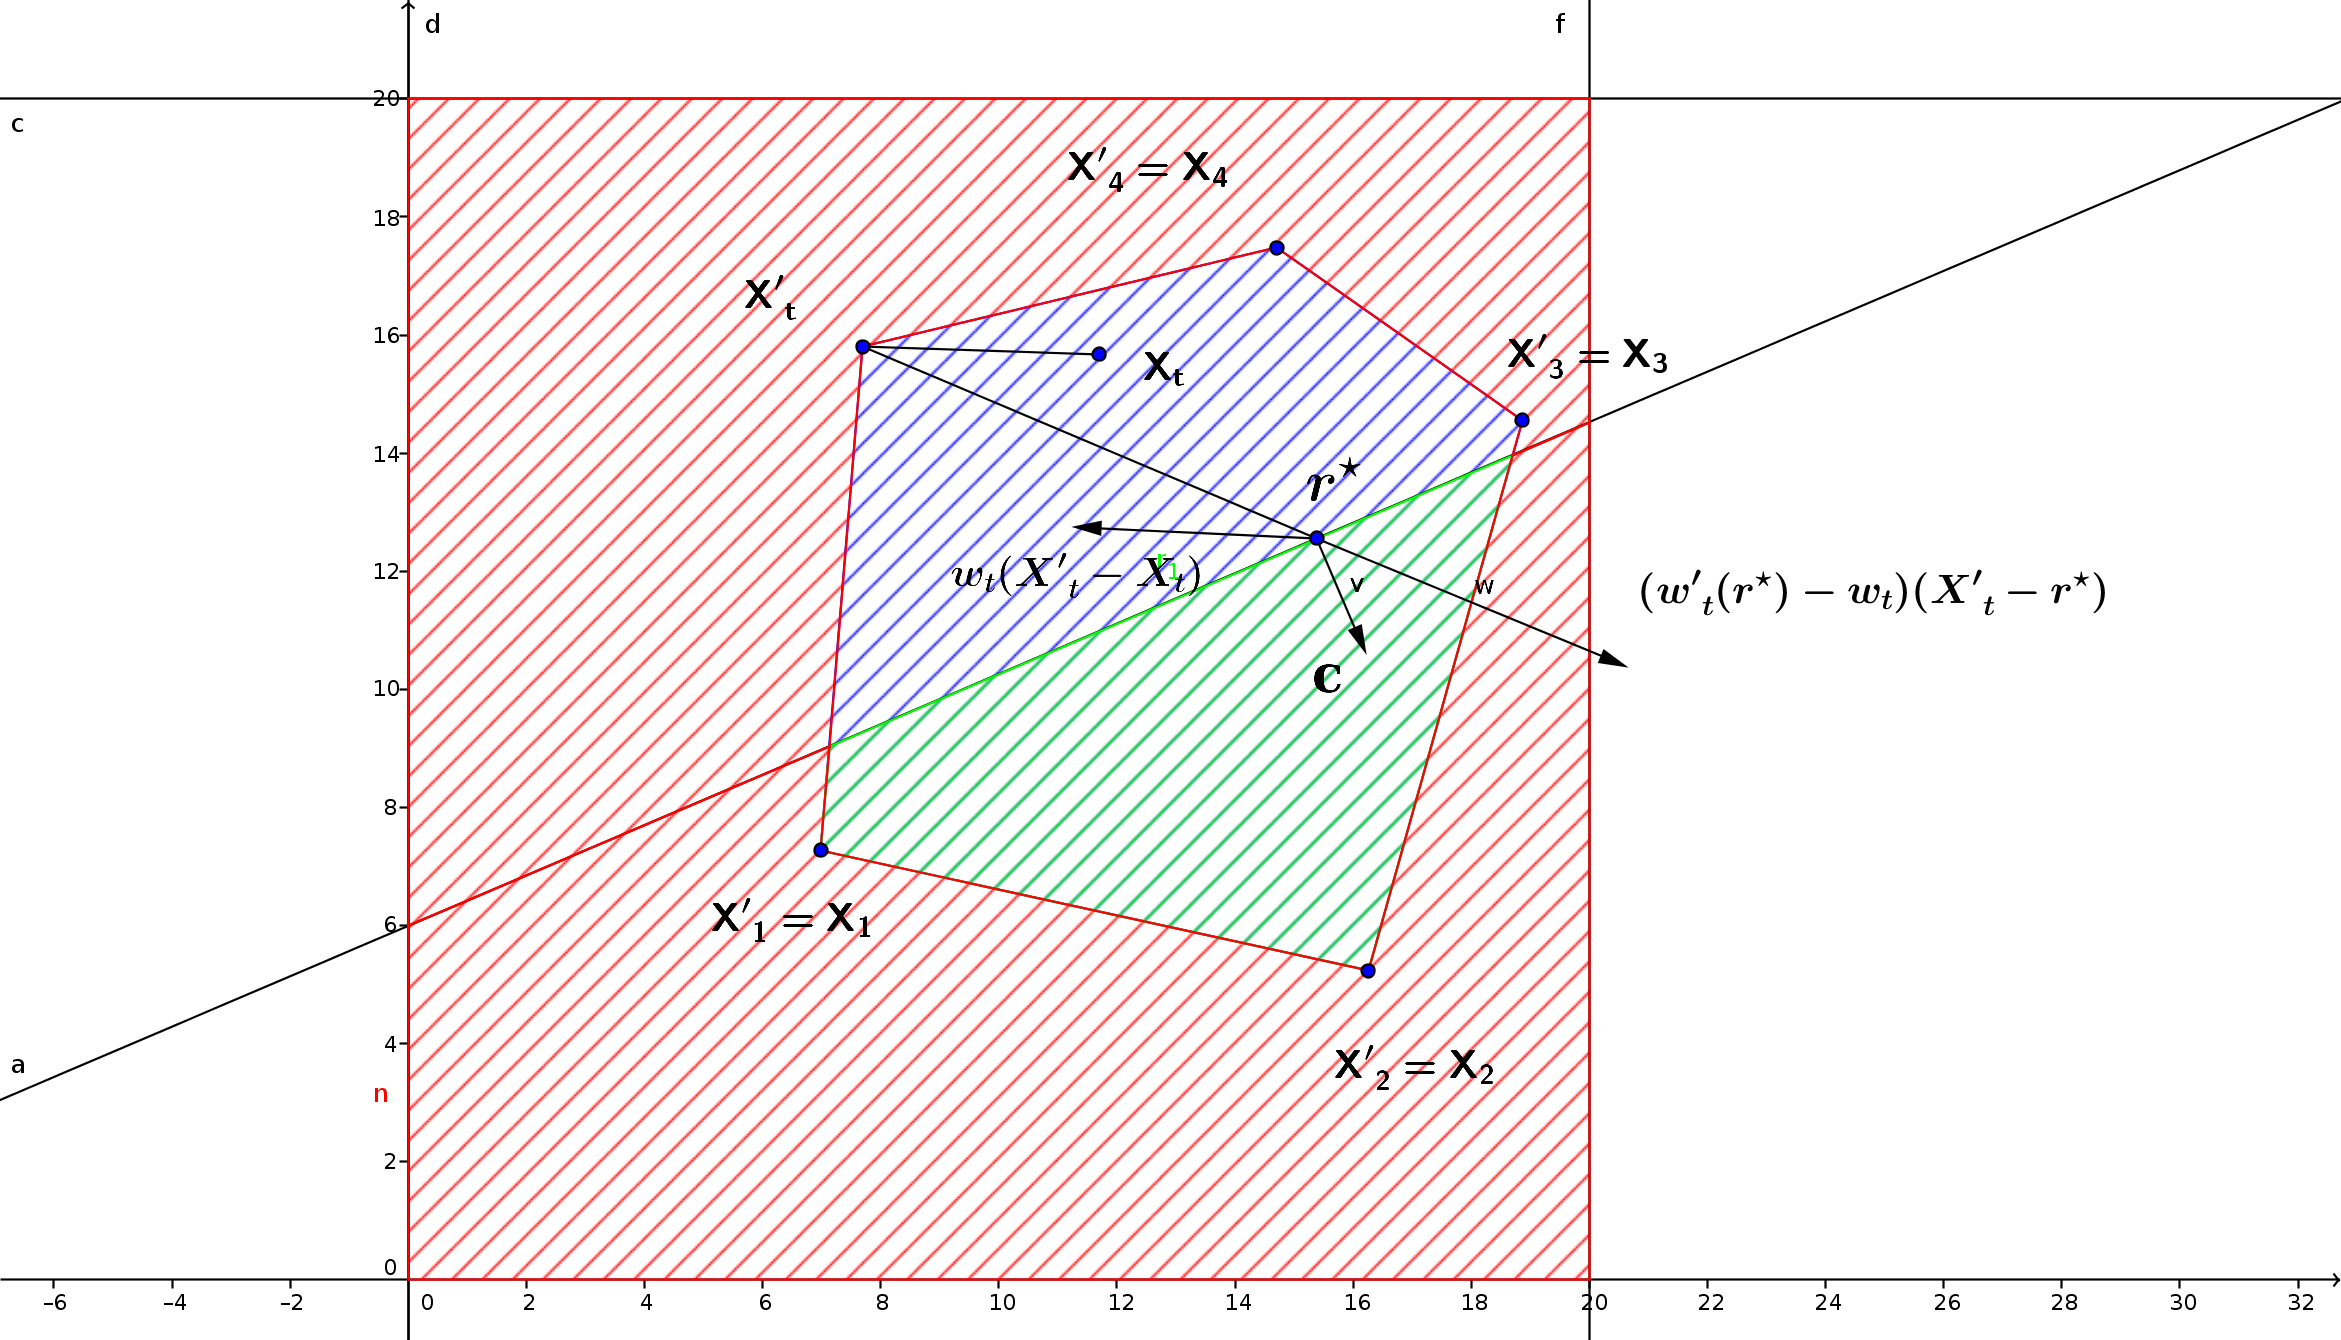
\includegraphics[width=0.7\textwidth]{../rapport/images/geogebra/Hyperplane.png}
        \end{figure}
        
\end{frame}

\begin{frame}{Cheating}
\framesubtitle{Example}
        \begin{exampleblock}{Question}
            How does a cheater determine which value to give his ratings in order to maximize (or minimize) a final rating? He can't!
        \end{exampleblock}
        
        \begin{figure}
            \centering
            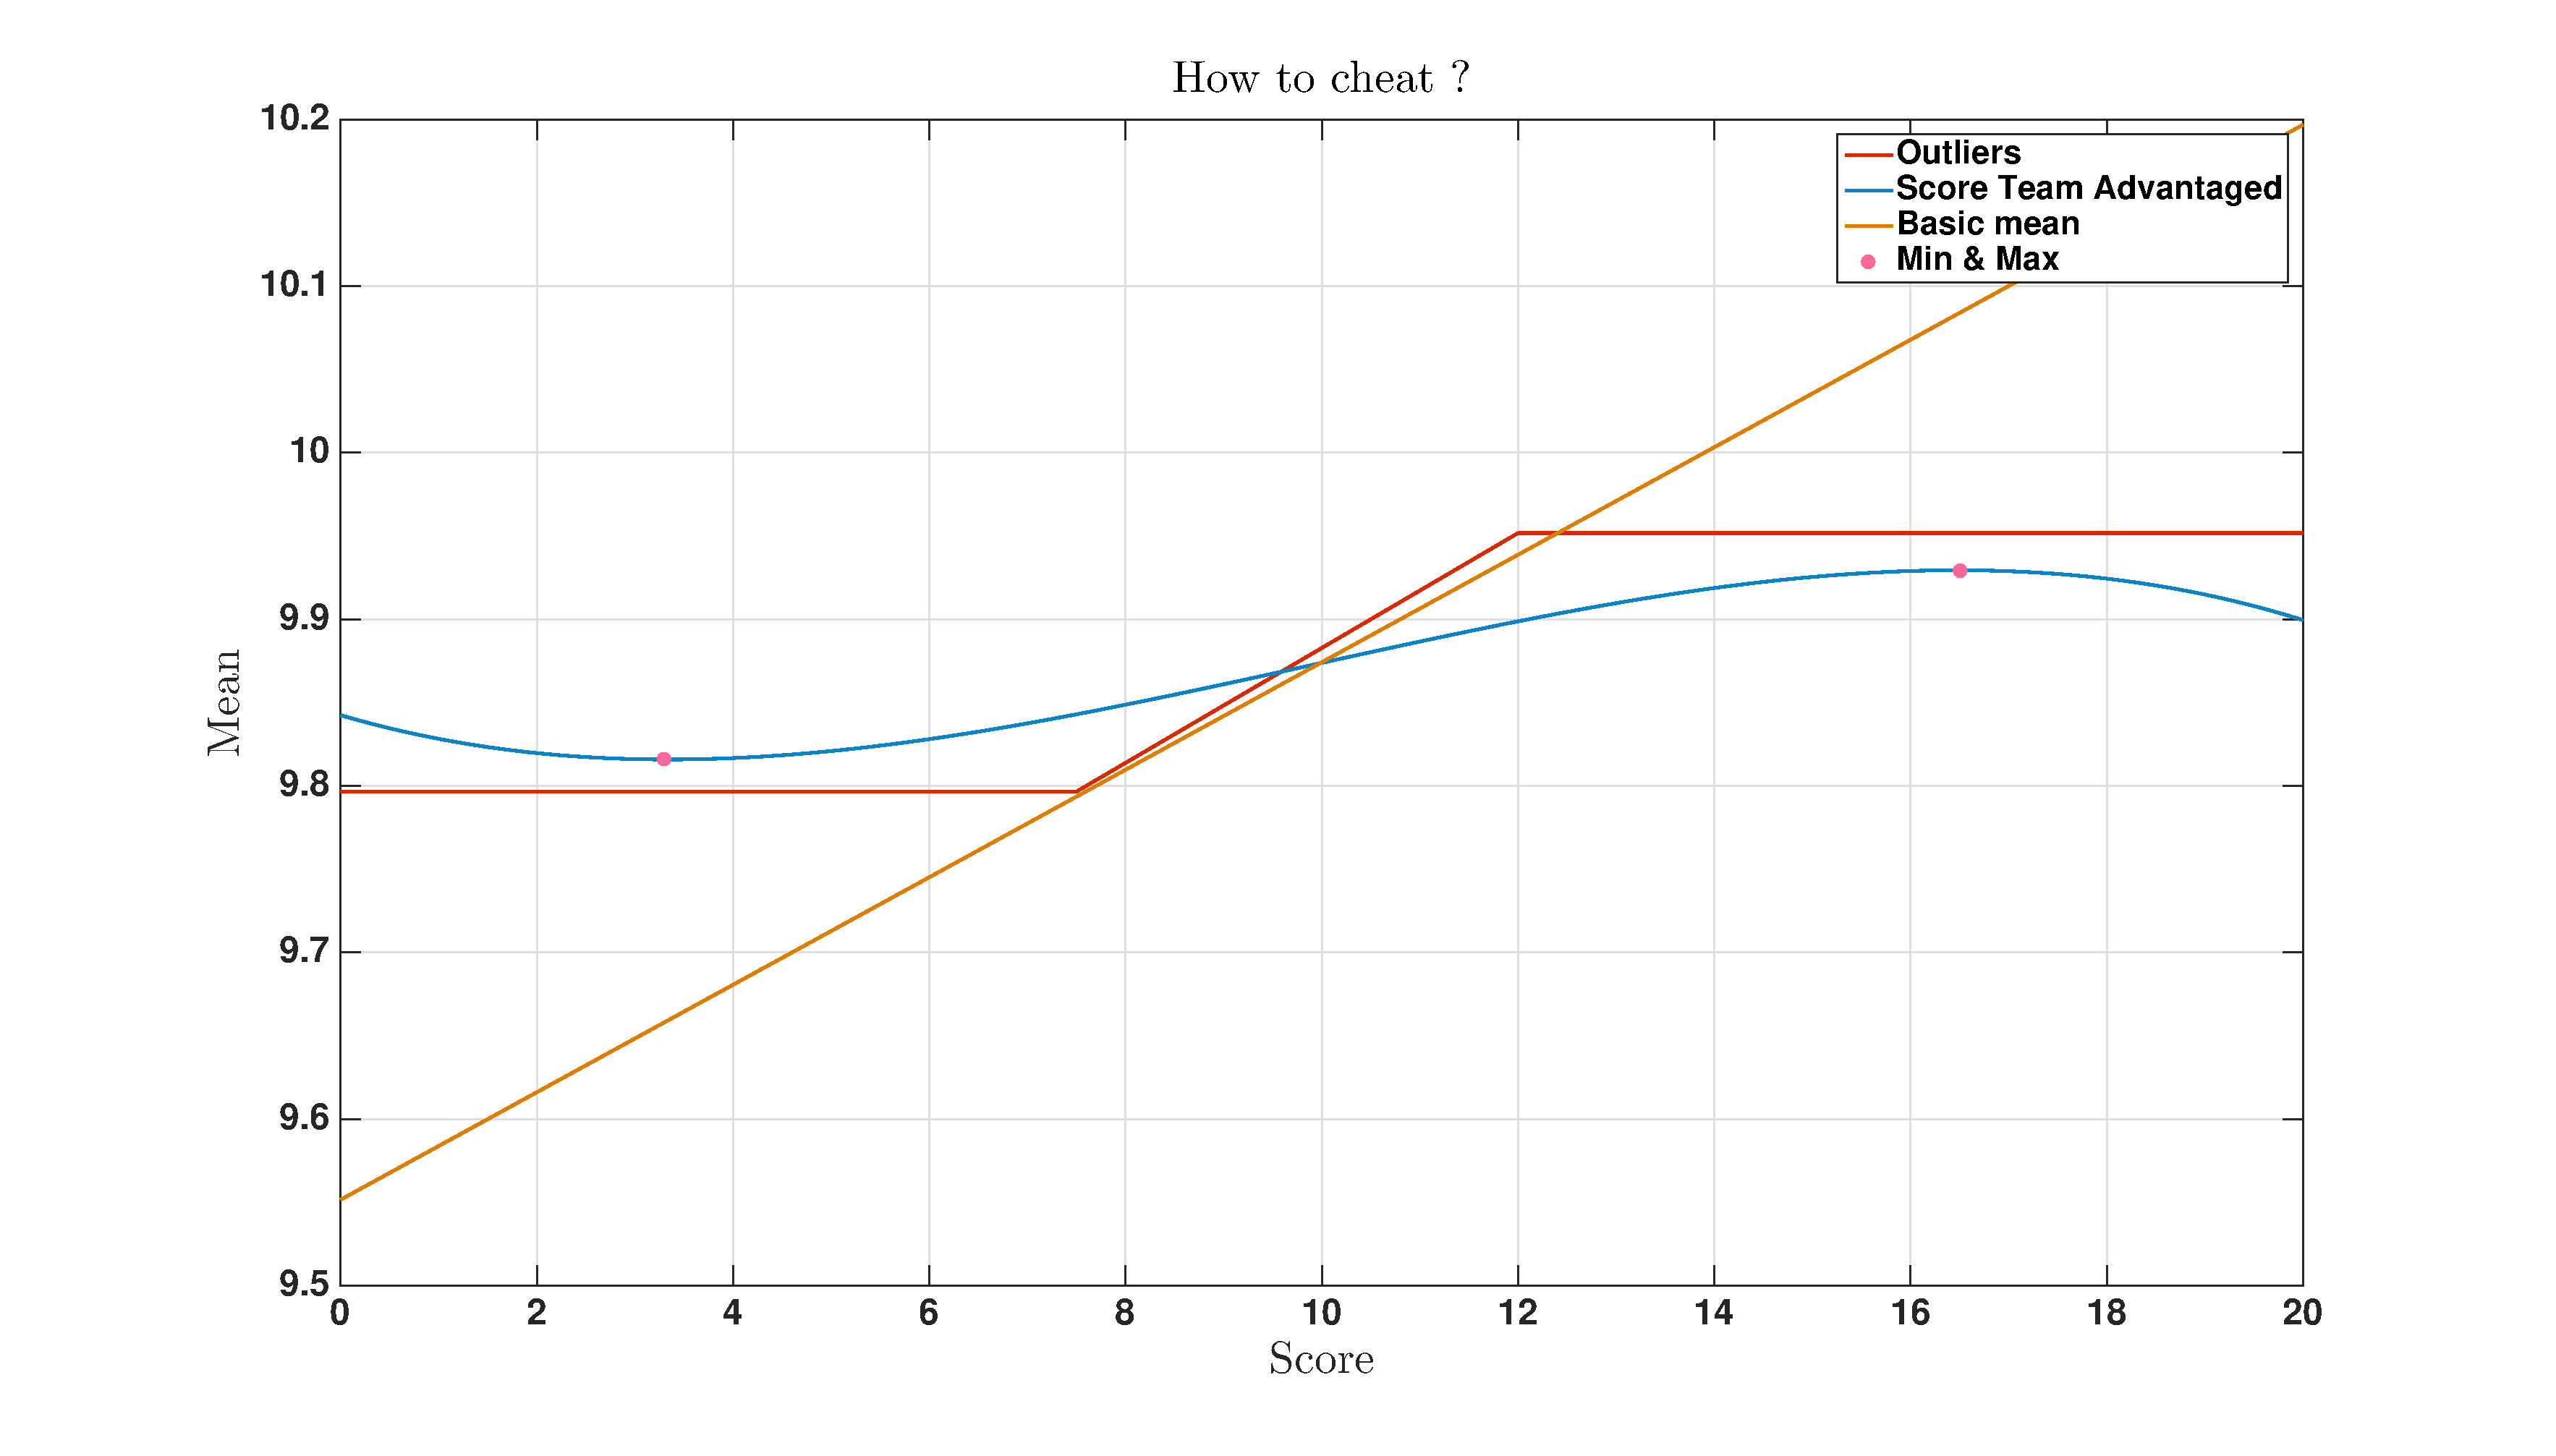
\includegraphics[width=\textwidth]{../rapport/images/cheaters/howto.eps}
        \end{figure}
\end{frame}

\begin{frame}{Application \rom{1}: MAP Scores}
\begin{itemize}
    \item Subset of \textit{MAP Scores}:
    \begin{itemize}
        \item \numprint{18} anonymized teachers :(
        \item \numprint{87} anonymized students :)
        \item \numprint{30} anonymzed courses :(
    \end{itemize}
    \item Issues
    \begin{itemize}
        \item Only one teacher rate a course !
        \item A course can not be a characteristic ! Why ?
        \item The result is the simple average because you can not compare one teacher with another...
        \item Some students doesn't try to take their exams...
    \end{itemize}
    \item Preprocessing
        \begin{itemize}
            \item Merge courses in two characteristics. Mandatory and optional courses.
            \item For each teacher we perform the simple average of the courses in each category.
            \item Delete students who do not try
        \end{itemize}
    \item Data are not sparse !
\end{itemize}
\end{frame}

\begin{frame}{Application \rom{1}: MAP Scores}
\begin{figure}[h!]
\centering
\begin{subfigure}[b]{0.24\textwidth}
    \centering
    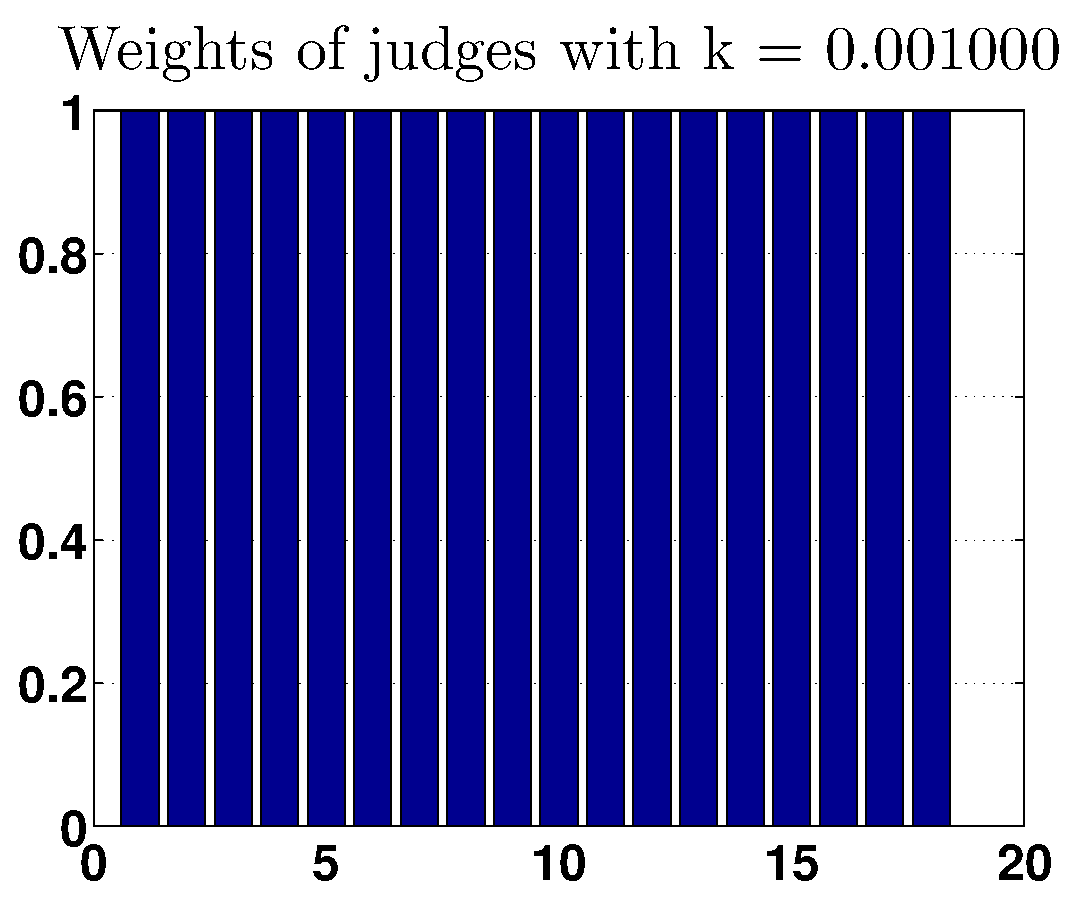
\includegraphics[width = \textwidth]{noPreprocess/weightsk10.eps}
\end{subfigure}
\begin{subfigure}[b]{0.24\textwidth}
    \centering
    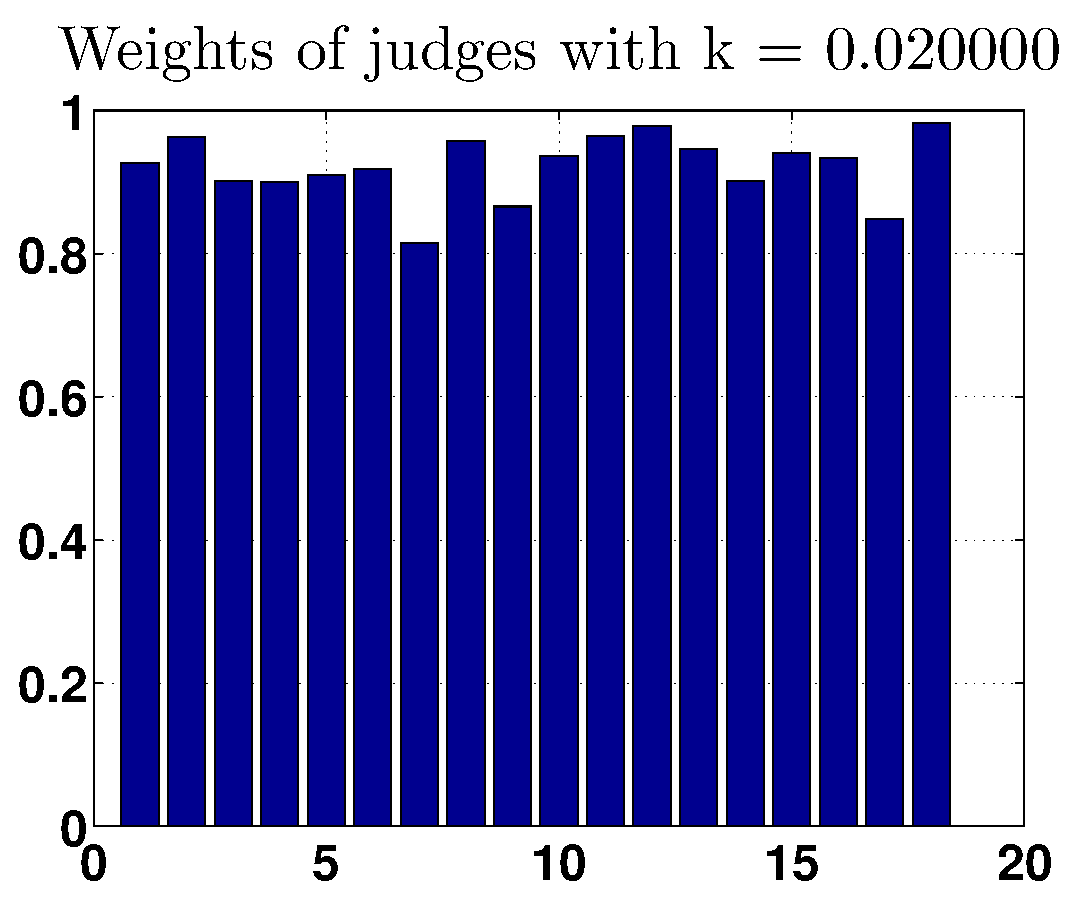
\includegraphics[width = \textwidth]{noPreprocess/weightsk200.eps}
\end{subfigure}
\begin{subfigure}[b]{0.24\textwidth}
    \centering
    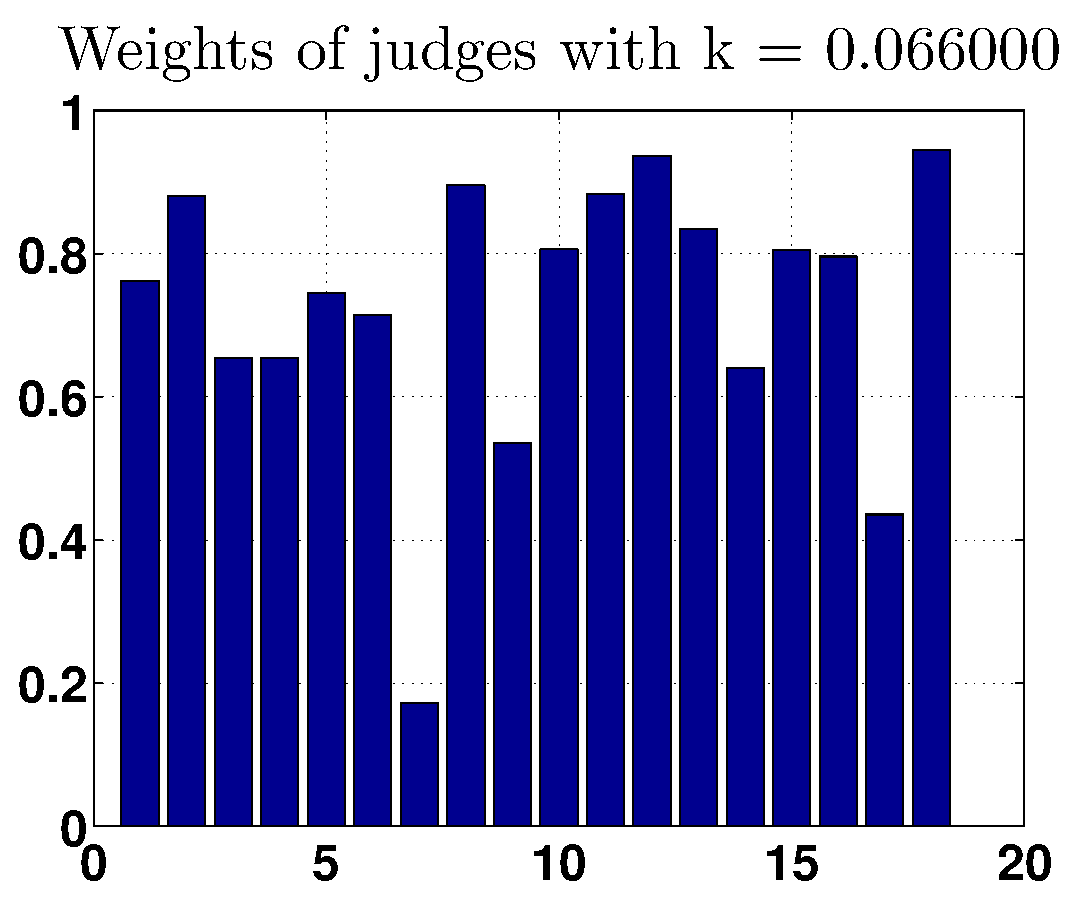
\includegraphics[width = \textwidth]{noPreprocess/weightsk660.eps}
\end{subfigure}
\begin{subfigure}[b]{0.24\textwidth}
\centering
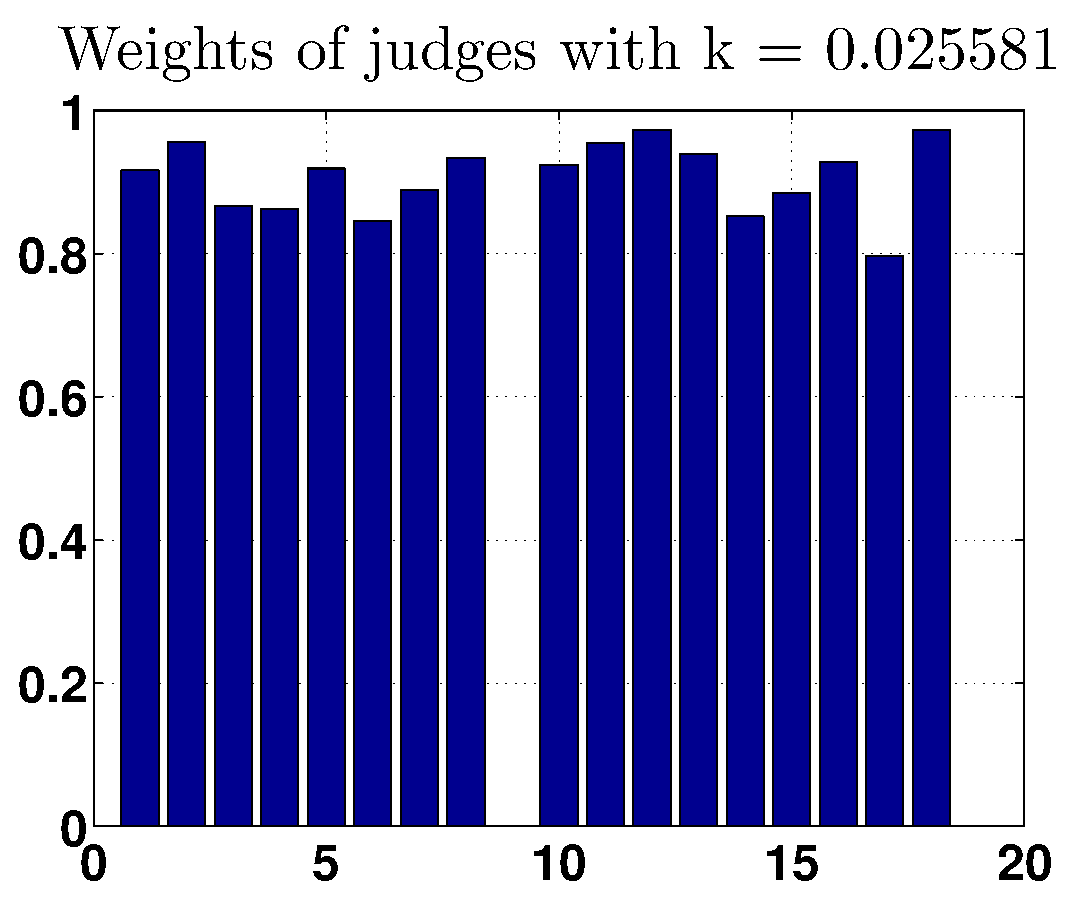
\includegraphics[width = \textwidth]{preprocess/ppweightsk3f9a31ee697a4e60.eps}
\end{subfigure}
\caption{Weights obtained with different values of k}
\end{figure}
\begin{itemize}
    \item We can always choose the value of k so that the least reliable judge has a weight zero.
    \item Order of judges does not change with k.
\end{itemize}
\end{frame}

\begin{frame}{Application \rom{1}: MAP Scores}
    \framesubtitle{Cheaters scenarios}
    \begin{itemize}
        \item Three stupid cheaters who would simply give a rating of 20 to the favoured students and the minimum acceptable note for disfavoured students.
        \item Three more subtle cheaters who, rather than giving 20 and 8 gave 19 and 9.
        \item Mixed the two behaviours, using one stupid cheater and two subtle cheaters.
    \end{itemize}
\end{frame}

\begin{frame}{Application \rom{1}: MAP Scores}
    \framesubtitle{Cheaters scenarios}
\begin{figure}[!ht]
\begin{subfigure}[b]{0.32\textwidth}
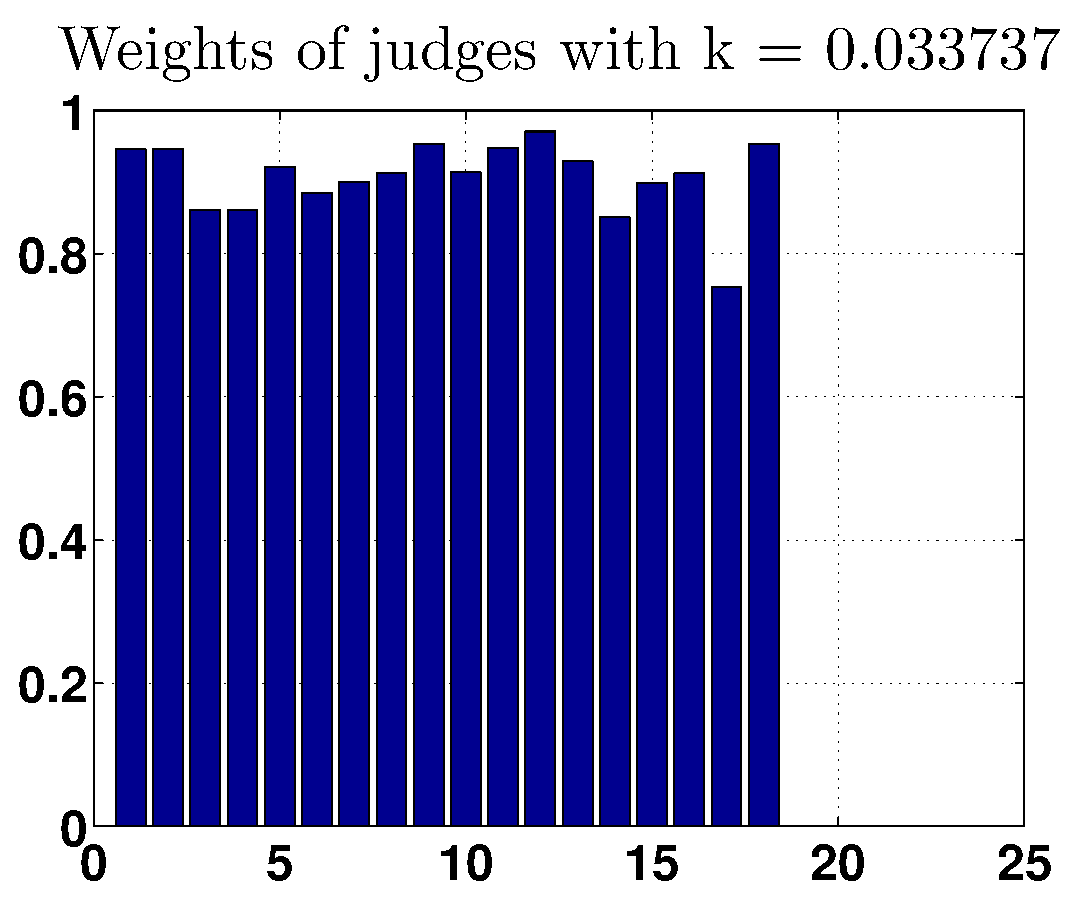
\includegraphics[width = \textwidth]{cheaters/chweightsStupid.eps}
\end{subfigure}
\begin{subfigure}[b]{0.32\textwidth}
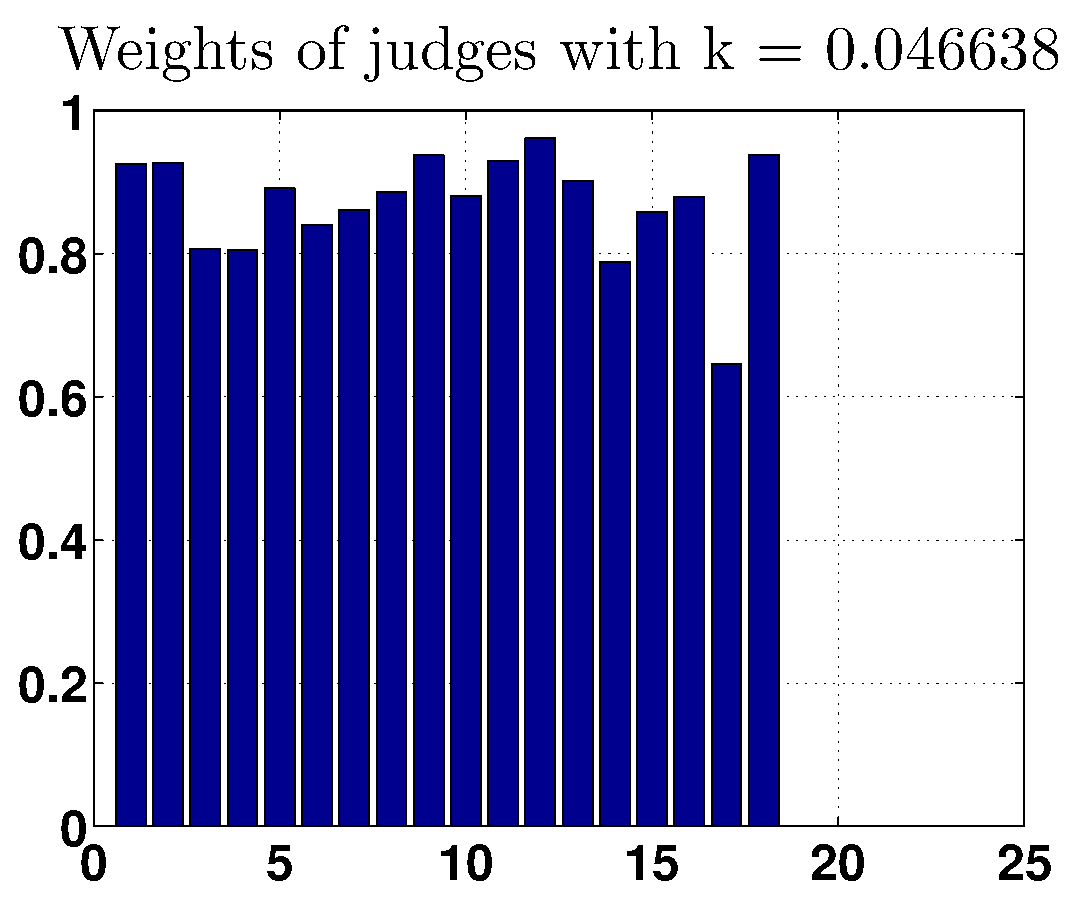
\includegraphics[width = \textwidth]{cheaters/chweightsSmart.eps}
\end{subfigure}
\begin{subfigure}[b]{0.32\textwidth}
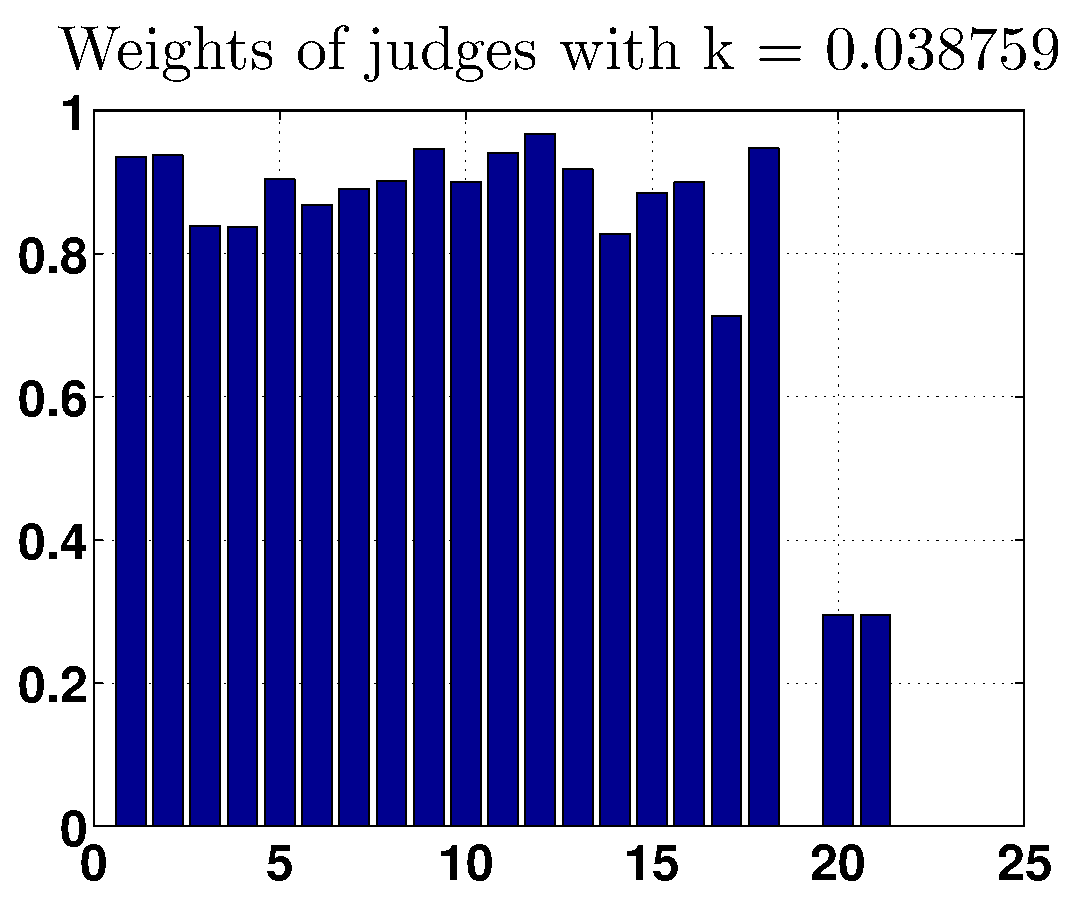
\includegraphics[width = \textwidth]{cheaters/chweightsMix.eps}
\end{subfigure}
\caption{Weights for the three scenario of cheaters\label{weightch}.}
\end{figure}
\end{frame}

\usebackgroundtemplate{%
    \tikz\node[opacity=0.1] {
\includegraphics[height=\paperheight]{images/tripadvisor.jpg}};
}
\begin{frame}{Application \rom{2}: Hotels}
\begin{itemize}
    \item Subset of \textit{TripAdvisor}:
    \begin{itemize}
        \item \numprint{1 169 410} users
        \item \numprint{12 773} hotels
        \item \numprint{10} characteristics rated between 0 and 5\\ (service, cleanliness, price, location, $\dots$)
    \end{itemize}
    \item Preprocessing:
    \begin{itemize}
        \item[Step 1:] Keep only the users who voted for at least 4 hotels
        \item[Step 2:] Keep only the hotels that have at least 2 votes
        \item[Step 3:] If some users have only three votes or less, go to step 1
    \end{itemize}
    \item After preprocessing:
    \begin{itemize}
        \item \numprint{20 024} users
        \item \numprint{308} hotels
        \item \numprint{9} characteristics
    \end{itemize}
    \item Data are very sparse !
    \item Unfortunately, we do not detect a specific behaviour :(
\end{itemize}
\end{frame}

\begin{frame}{Application \rom{2}: Hotels with spammers (1)}
    Added 20 spammers giving always 0 except for their preferred hotel, which they rated 5 on all characteristics.
            \begin{figure}
            \centering
            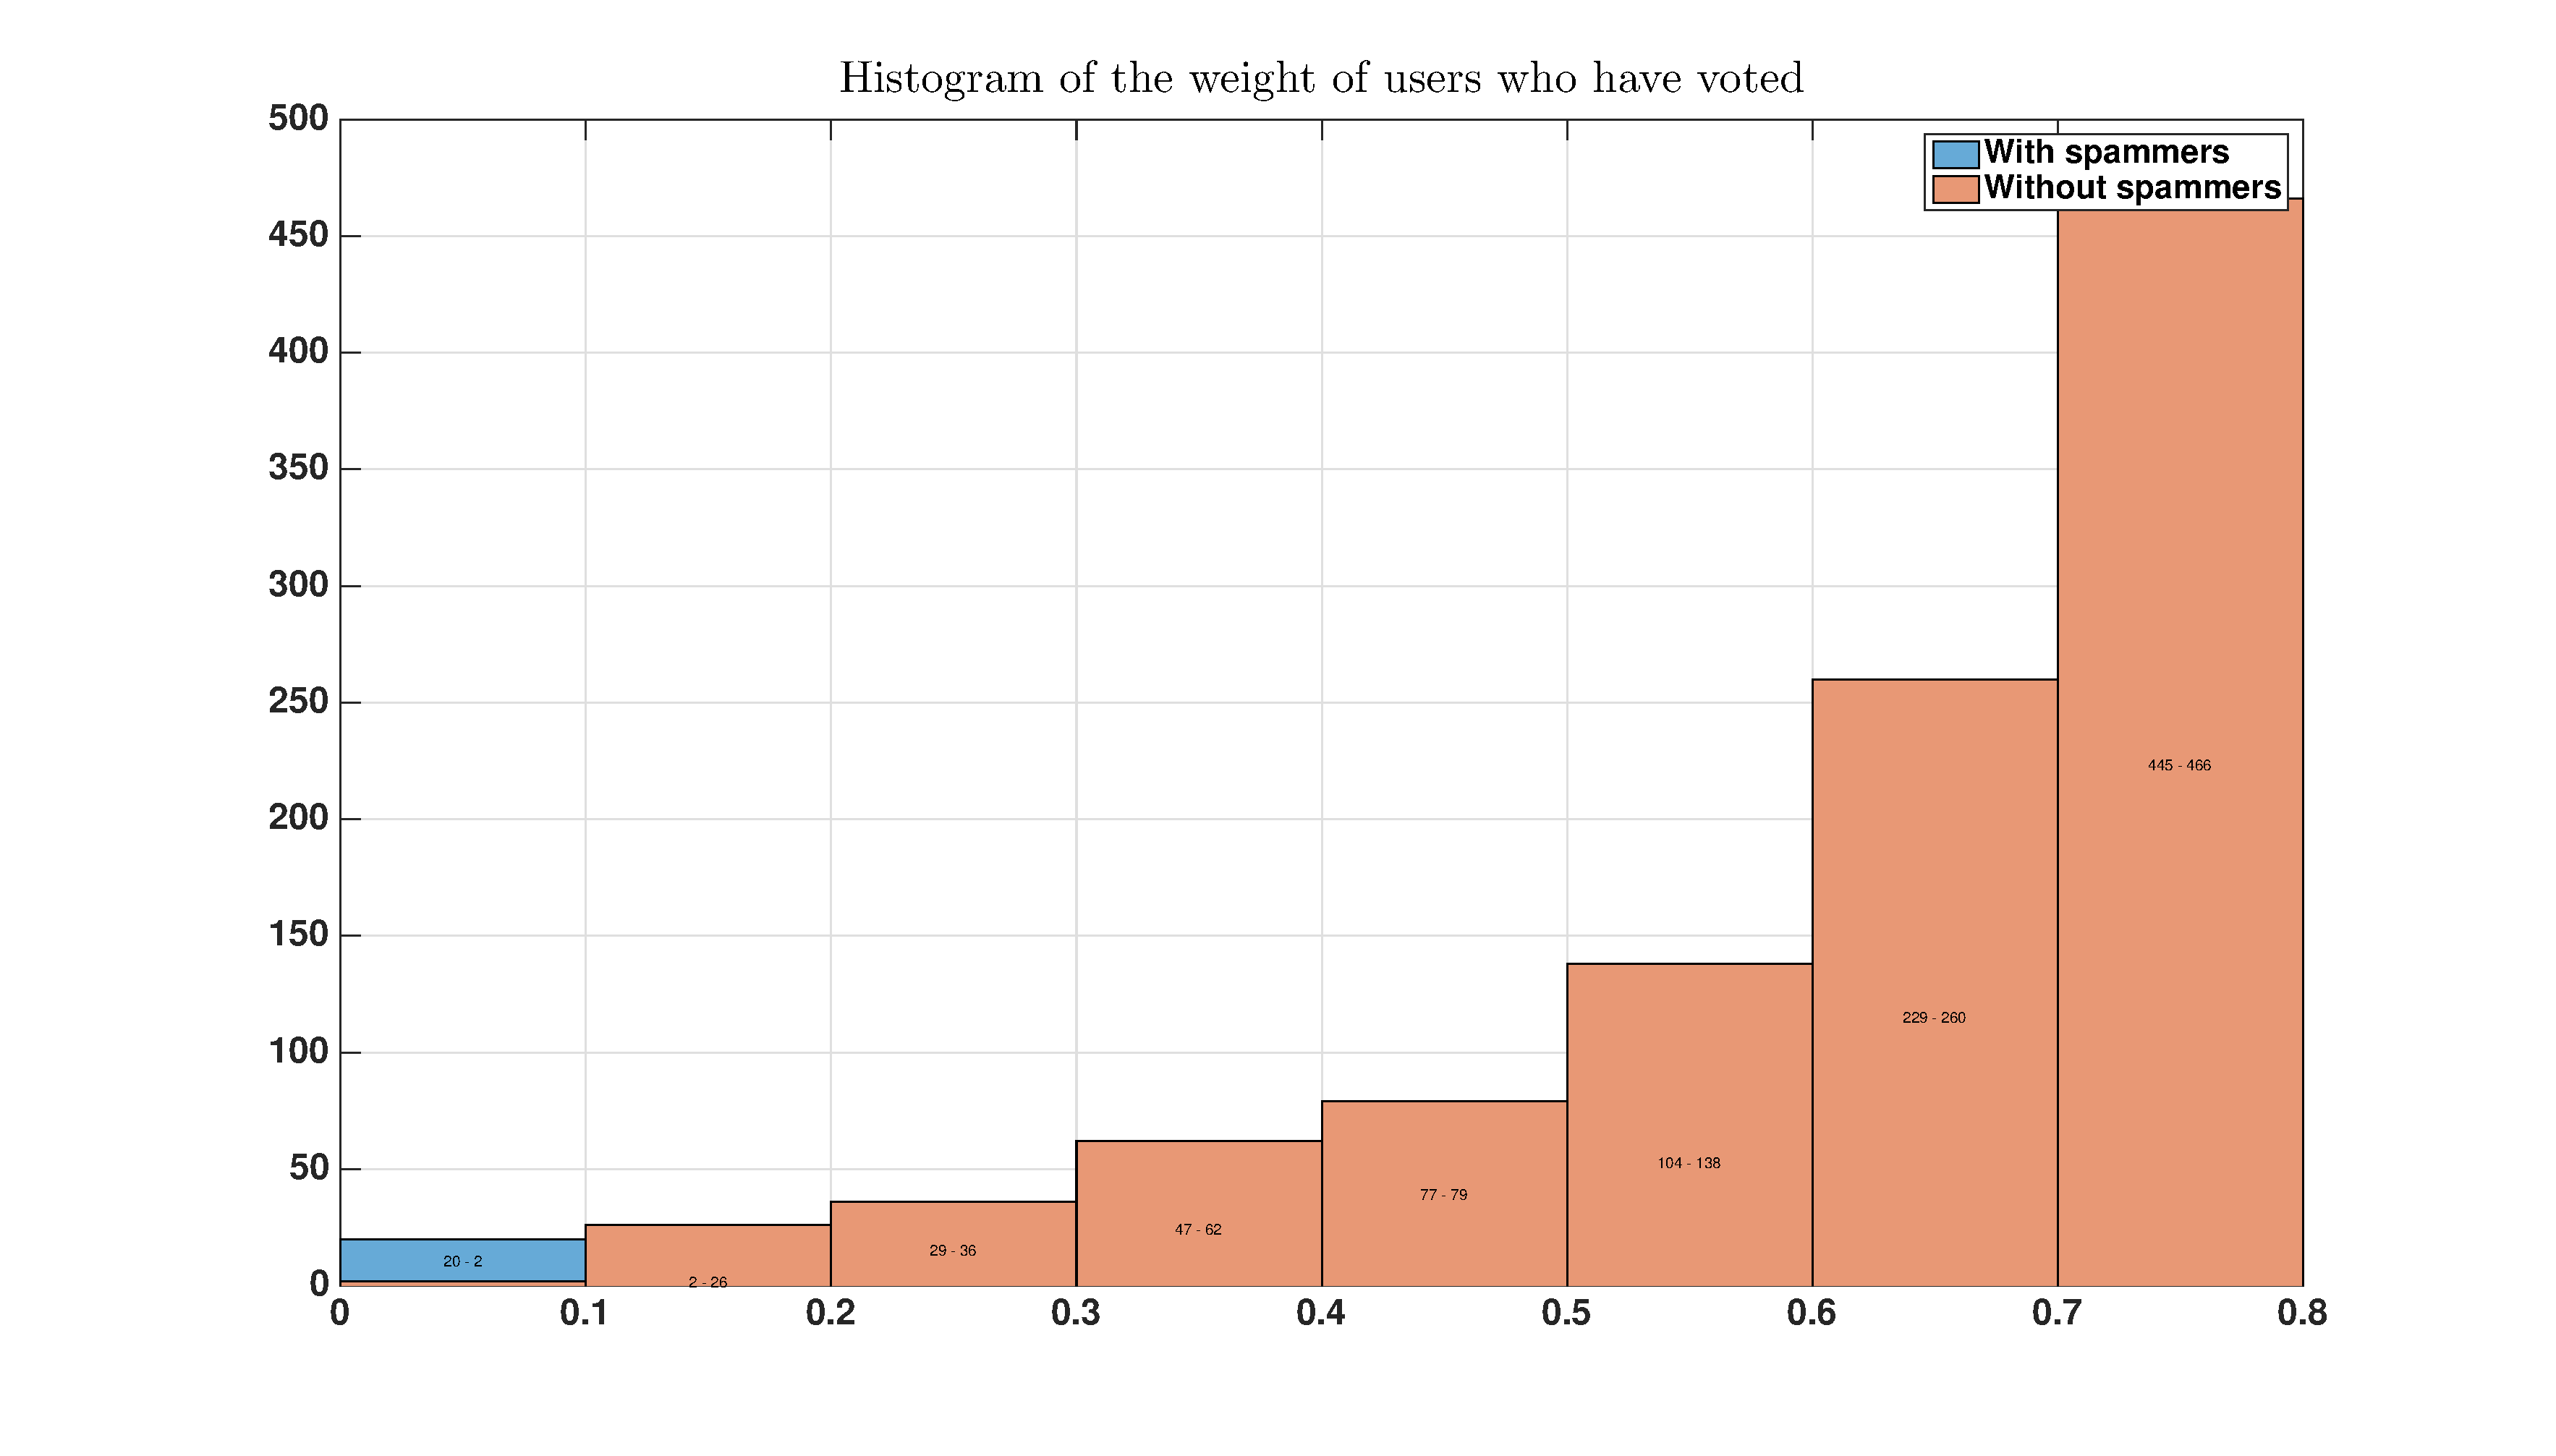
\includegraphics[width=\textwidth]{../rapport/images/hotels/not_random_cheaters.eps}
        \end{figure}
\end{frame}

\begin{frame}{Application \rom{2}: Hotels with spammers (2)}
    We now added to the original data set one spammer per hotel giving always 0 except for their own hotel, which they rated 5.
            \begin{figure}
            \centering
            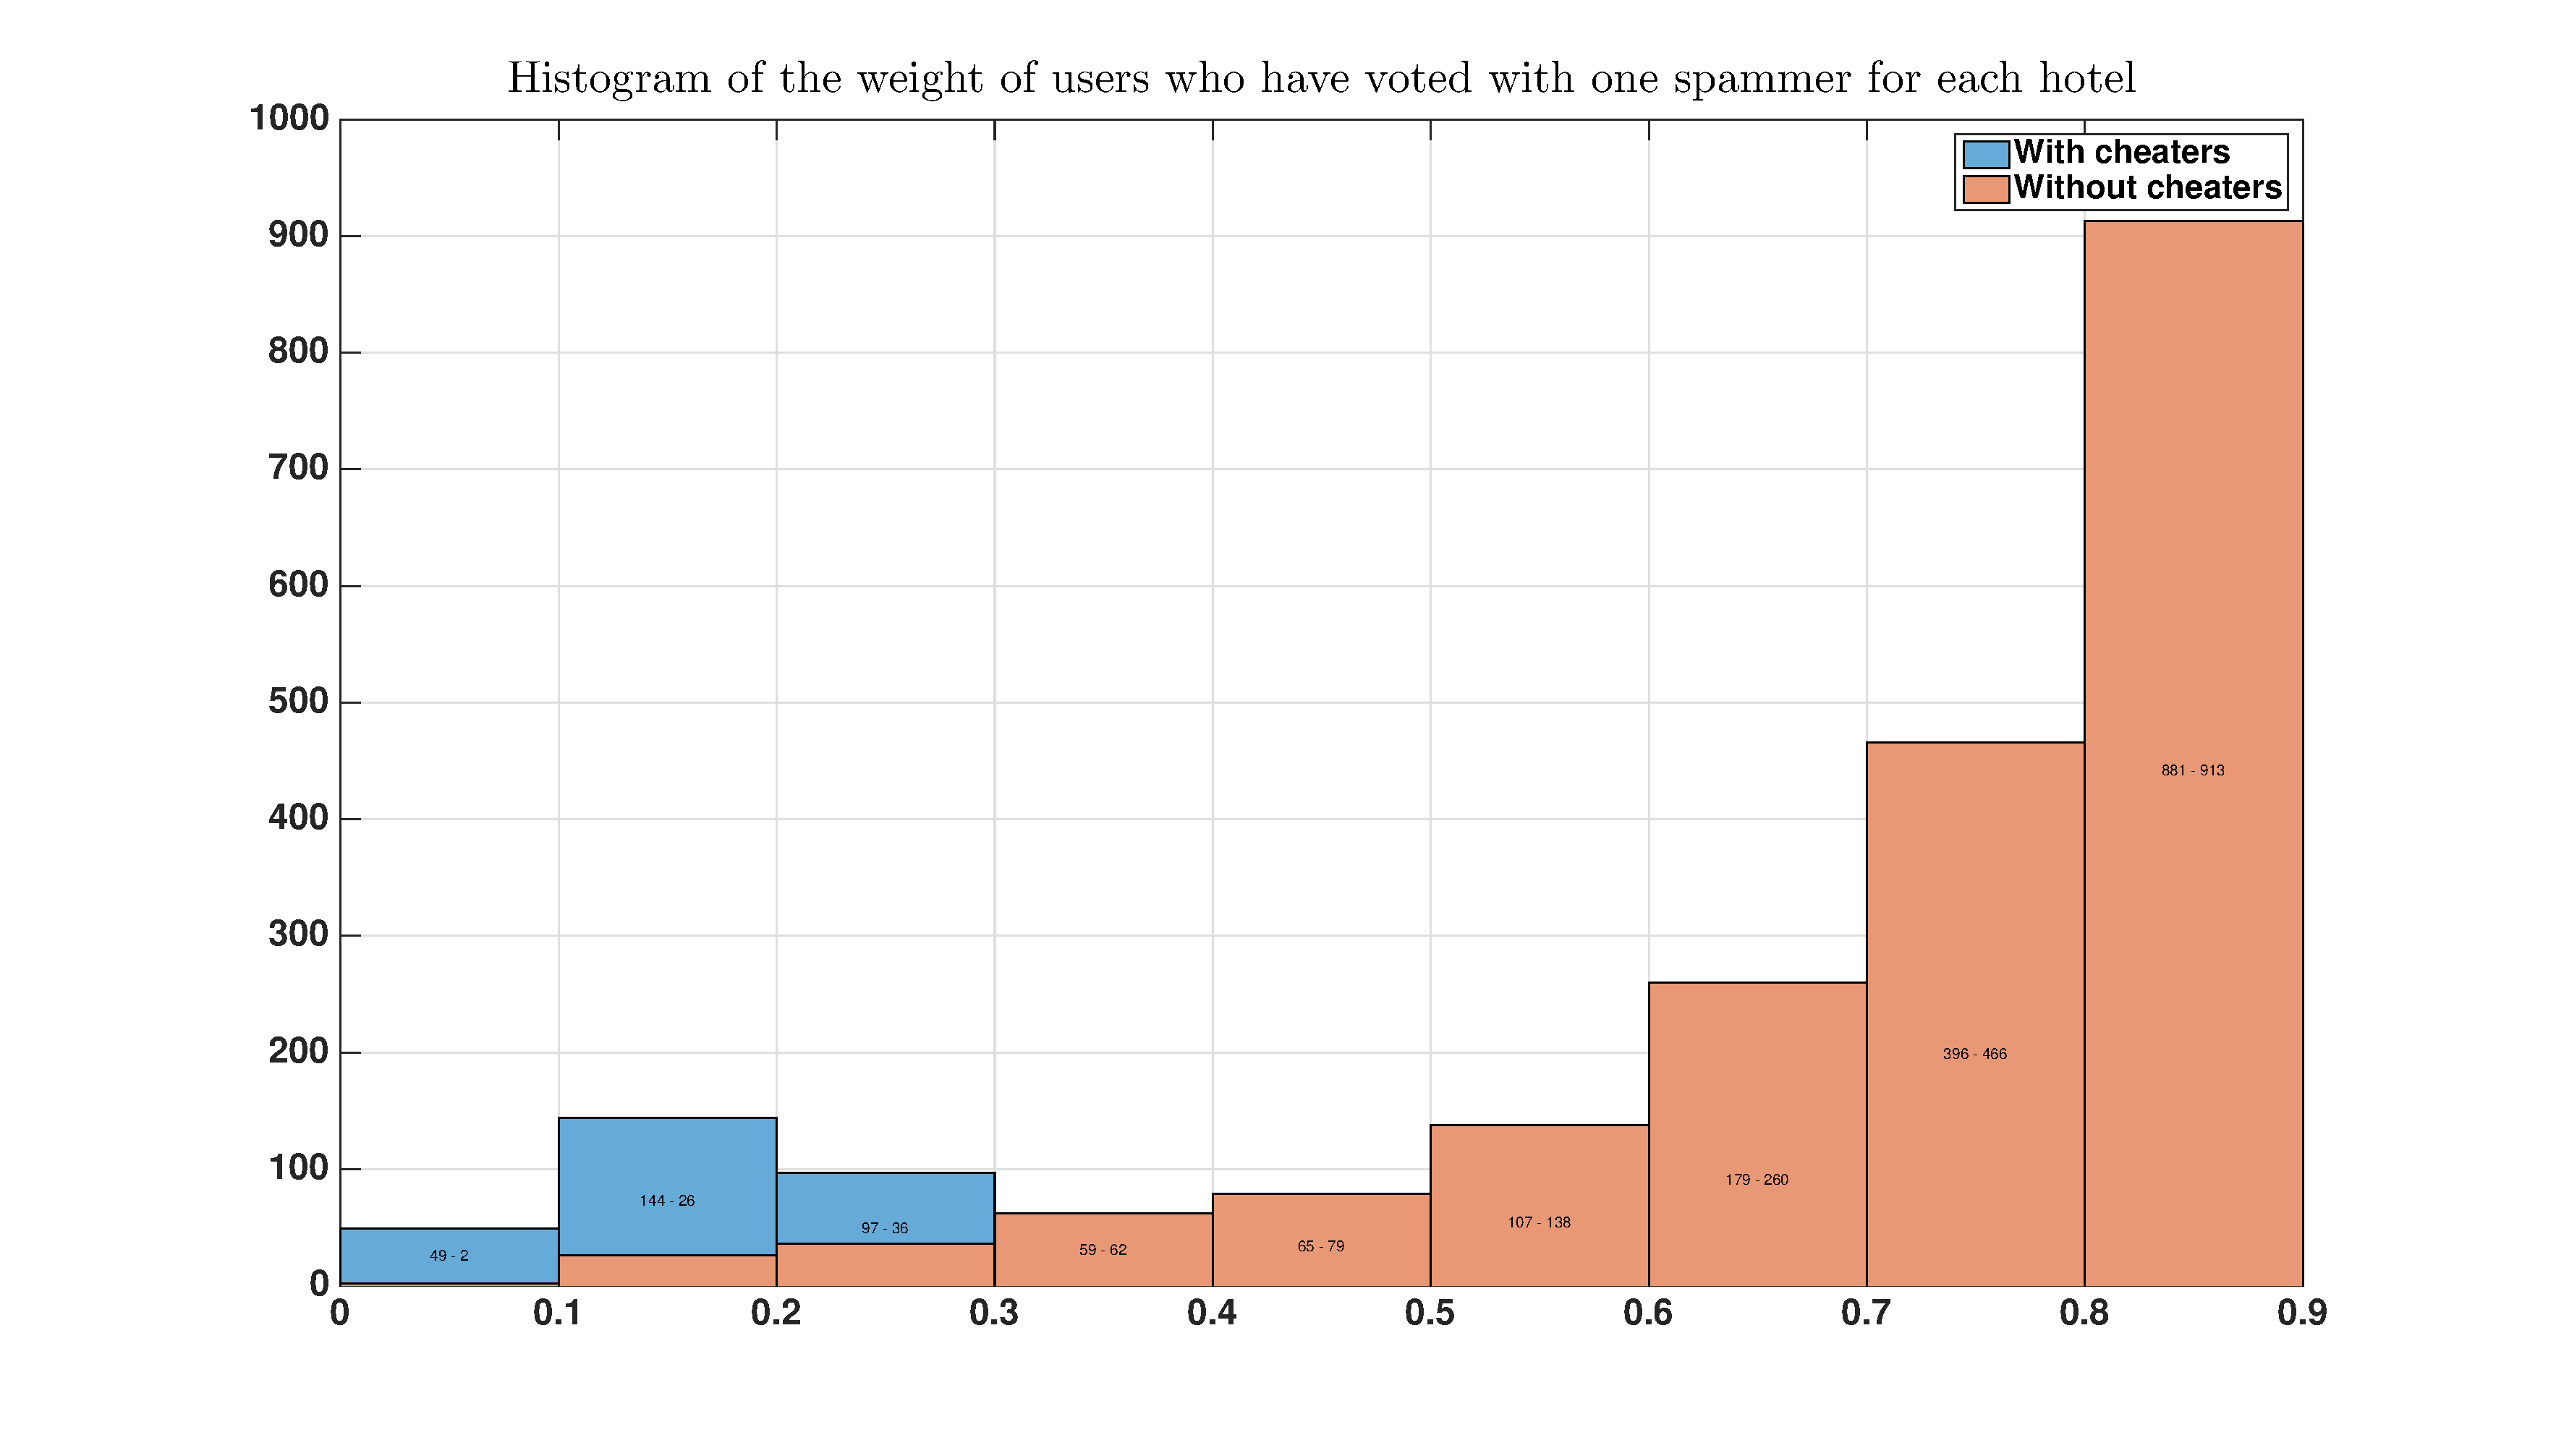
\includegraphics[width=\textwidth]{../rapport/images/hotels/not_random_each_hotels.eps}
        \end{figure}
\end{frame}

\usebackgroundtemplate{}
\begin{frame}{Conclusion}

\end{frame}